\documentclass{article}
\usepackage[utf8]{inputenc}
\usepackage{blindtext}
\usepackage{enumitem}
\usepackage{graphicx}
\usepackage{hyperref}
\usepackage{titletoc}
\usepackage{float} 

\graphicspath{ {images/} }

\hypersetup{colorlinks=true,
urlcolor=blue,
linkcolor=black}

\title{ \begin{center}
					
\includegraphics[scale=0.6]{./images/FEUPlogo}
				\end{center}
				\textbf{Werewolves of Miller's Hollow}}
\author{Miguel Lira Barbeitos Luís - up201405324\\
		Miriam Cristiana Meireles Campos Gonçalves - up201403441\\
		Paulo Sérgio Silva Babo - up201404022}
\date{03 Janeiro, 2018}
\begin{document}

\begin{titlepage}
	\centering
	
\includegraphics[width=1\textwidth]{./images/FEUPlogo}\par\vspace{1cm}
	{\huge\bfseries Fashion Show \par}
	\vspace{2cm}
	{\scshape\Large Relatório Final\par}
	\vspace{1.5cm}
	{\large\bfseries Métodos Formais em Engenharia de Software\par}
	\vspace{0.7cm}
	{\scshape\normalsize  Mestrado Integrado em Engenharia Informática e Computação \par}
	\vspace{1.5cm}
	{\Large\itshape Grupo\textunderscore04 Turma\textunderscore01 
	\par Miguel Lira Barbeitos Luís - up201405324 \par
	Miriam Cristiana Meireles Campos Gonçalves - up201403441 \par
	Paulo Sérgio Silva Babo - up201404022\par}

	\vfill
% Bottom of the page
	{\large \today\par}
\end{titlepage}
\thispagestyle{empty}

\newpage

\tableofcontents

\newpage

\section{Descrição Informal do Sistema e Lista de Requisitos}
\subsection{Descrição Informal do Sistema}
\subsection{Lista de Requisitos}

\section{Modelo UML}
\subsection{Modelo de Casos de Uso}
\subsection{Diagrama de Classes}
\begin{figure}[H]
\centering
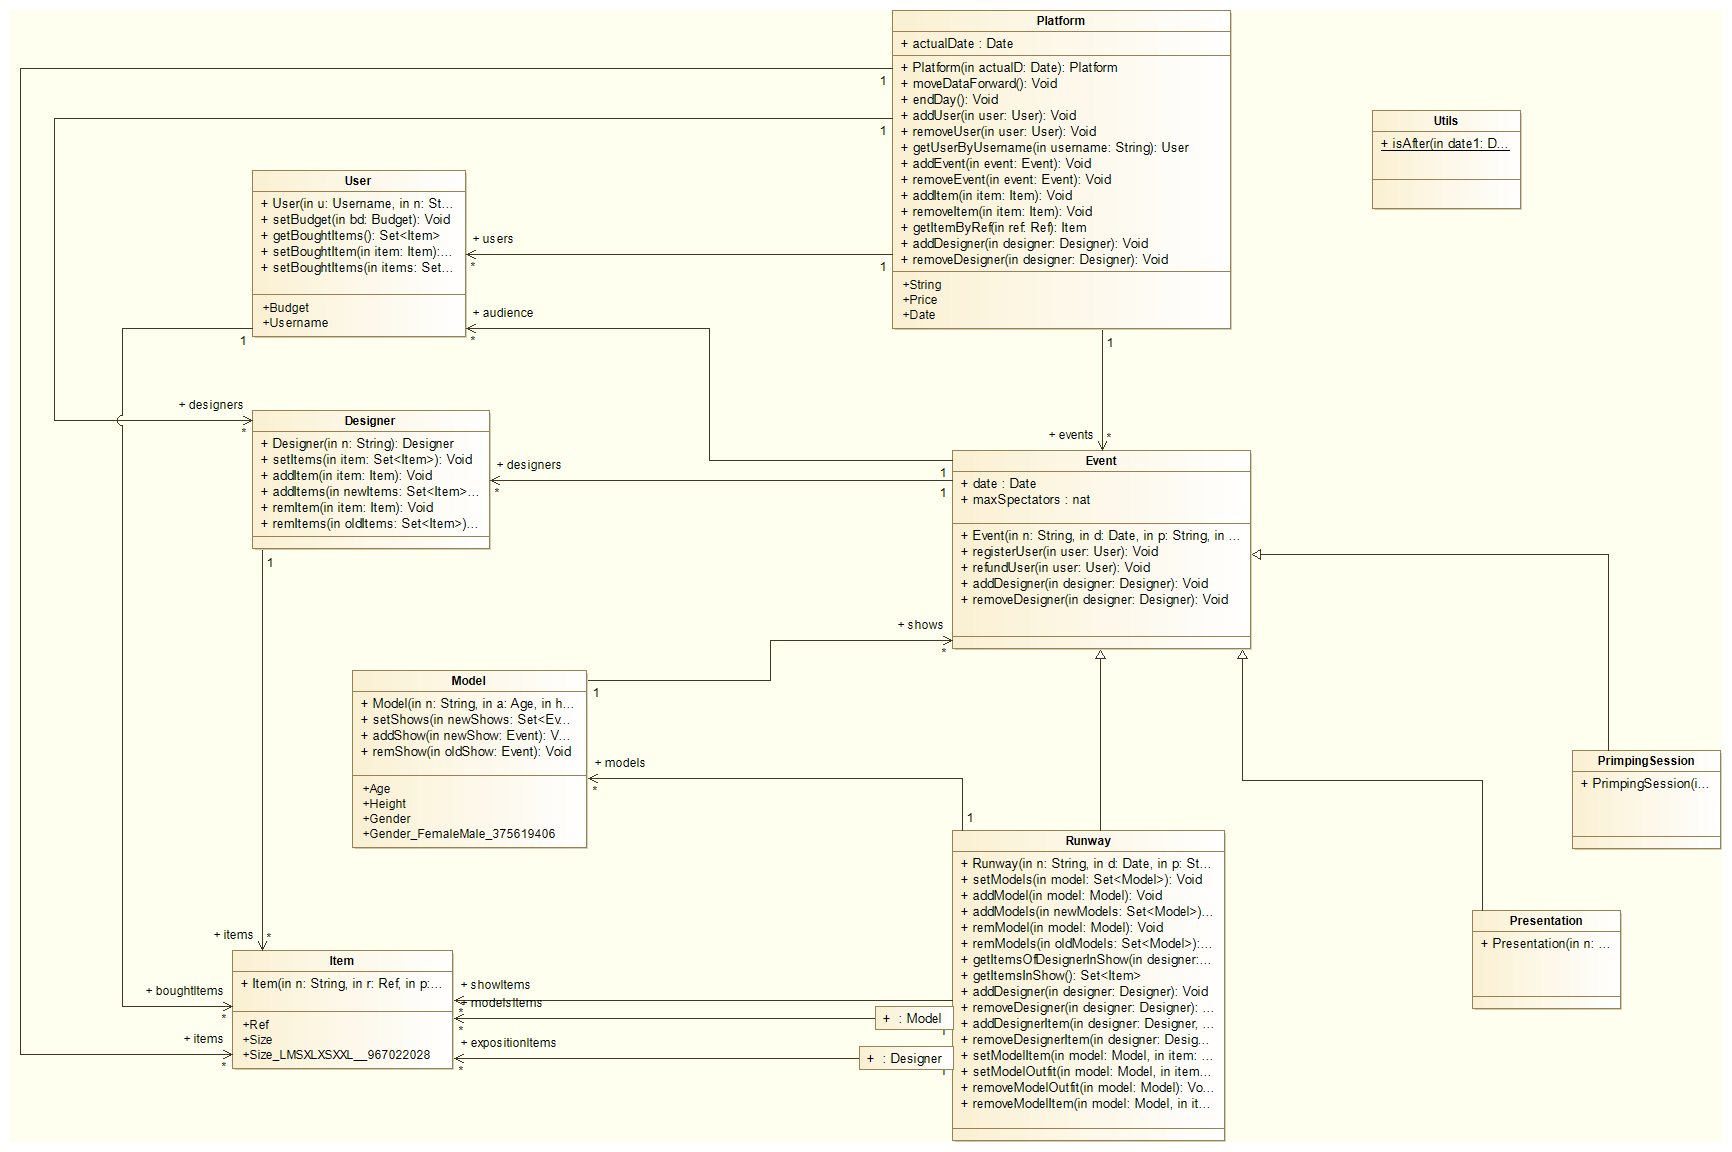
\includegraphics[width=160mm,height=150mm]{./images/class_diagram.png}
\caption{Diagrama de classes}
\label{fig:method}
\end{figure}
		
\section{Modelo Formal VDM++}
\subsection{Class FashionShow}
\subsection{Class Model}
\subsection{Class Designer}

\section{Modelo de Validação}
\subsection{Class Test}

\section{Modelo de Verificação}

\section{Geração de código}

\section{Conclusões}
\section{Referências}
\subsection{Bibliografia}
\noindent
(1) Peter Gorm Larsen, Kenneth Lausdahl, Nick Battle, John Fitzgerald, Sune Wolff, Shin Sahara, Marcel Verhoef, Peter W. V. Tran-Jørgensen, Tomohiro Oda, Paul Chisholm, Overture "VDM-10 Language Manual"\\

\noindent
(2) Peter Gorm Larsen, John Fitzgerald, Sune Wolff, Nick Battle, Kenneth Lausdahl, Augusto Ribeiro, Kenneth Pierce, Victor Bandur, "Tutorial for Overture/VDM++"\\

\noindent
(3) Sarit Kraus, Katia Sycara, Amir Evenchik, "Reaching agreements through argumentation: a logical model and implementation"\\

\noindent
(4) Peter Gorm Larsen, Kenneth Lausdahl, Peter Jørgensen, Joey Coleman, Sune Wolff and Luís Diogo Couto Aarhus University, Department of Engineering Finlandsgade 22, DK-8000 Aarhus C, Denmark, "Overture VDM-10 Tool Support: User Guide"\\
\subsection{Software}

Eclipse \\
\vspace{3mm}\url{http://www.eclipse.org/} \\
Overture \\
\vspace{3mm}\url{http://overturetool.org/} \\
Modelio \\
\vspace{3mm}\url{https://www.modelio.org/} \\
\end{document}